%%%% Proceedings format for most of ACM conferences (with the exceptions listed below) and all ICPS volumes.
%\documentclass[sigconf]{acmart}
\documentclass[sigchi]{acmart} %pedro changed for camera ready

%%%% As of March 2017, [siggraph] is no longer used. Please use sigconf (above) for SIGGRAPH conferences.

%%%% Proceedings format for SIGPLAN conferences 
% \documentclass[sigplan, anonymous, review]{acmart}

%%%% Proceedings format for SIGCHI conferences
% \documentclass[sigchi, review]{acmart}

%%%% To use the SIGCHI extended abstract template, please visit
% https://www.overleaf.com/read/zzzfqvkmrfzn


\usepackage{booktabs} % For formal tables

% custom packages
\usepackage{enumitem}
\usepackage{hyperref}
\usepackage[colorinlistoftodos,backgroundcolor=white,prependcaption,textsize=tiny,linecolor=black]{todonotes}

\makeatletter
\providecommand\@dotsep{5}
\def\listtodoname{List of Todos}
\def\listoftodos{\@starttoc{tdo}\listtodoname}
\makeatother

\usepackage{xcolor}

\newcommand\missing[1]{\textcolor{red}{<#1>}}
\newcommand\missingRef{\textcolor{red}{[REF]}}


% Copyright
% \setcopyright{none}
%\setcopyright{acmcopyright} %pedro changed for camera ready
\setcopyright{acmlicensed}
%\setcopyright{rightsretained} %was bfore
%\setcopyright{usgov}
%\setcopyright{usgovmixed}
%\setcopyright{cagov}
%\setcopyright{cagovmixed}

% DOI
%\acmDOI{10.475/123_4}

% ISBN
%\acmISBN{123-4567-24-567/08/06}

%Conference
%\acmConference[]{}{}{
% }
%\acmYear{}
%\copyrightyear{}
%\acmArticle{}
%\acmPrice{}


\begin{document}
\raggedbottom
\title[Detecting Visuo-Haptic Mismatches in VR using ERPs]{Detecting Visuo-Haptic Mismatches in Virtual Reality using the Prediction Error Negativity of Event-Related Brain Potentials}

%\titlenote{Produces the permission block, and
%  copyright information}
%\subtitle{Prediction Mismatches In Haptic VR (Comparing Different Sensory Stimulation Channels)}
%\subtitlenote{The full version of the author's guide is available as \texttt{acmart.pdf} document}

\author{Lukas Gehrke}
%\authornote{These authors contributed equally to this research.}
\email{lukas.gehrke@tu-berlin.de}
\orcid{10000-0003-3661-1973}
\affiliation{%
  \institution{Technical University of Berlin}
  \city{Berlin}
  \country{Germany}
}

\author{Sezen Akman}
%\authornotemark[1]
\email{sezen.akman@campus.tu-berlin.de}
\affiliation{%
  \institution{Technical University of Berlin}
  \city{Berlin}
  \country{Germany}
}

\author{Pedro Lopes}
%\authornotemark[1]
\authornote{Author affiliated also with Hasso Plattner Institute, Germany.}
\email{pedrolopes@cs.uchicago.edu}
\orcid{0000-0001-6527-7084}
\affiliation{%
  \institution{University of Chicago}
  \city{Chicago}
  \state{Illinois}
  \country{USA}
}

\author{Albert Chen}
\email{albertc1@uchicago.edu}
\affiliation{%
  \institution{University of Chicago}
  \city{Chicago}
  \state{Illinois}
  \country{USA}
}

\author{Avinash Kumar Singh}
\email{avinash.singh@uts.edu.au}
\affiliation{%
  \institution{National Chiao Tung University}
  \city{Hsinchu}
  \country{Taiwan}
}

\author{Hsiang-Ting Chen}
\email{Tim.Chen@uts.edu.au}
\affiliation{%
  \institution{University of Technology Sydney}
  \city{Sidney}
  \country{Australia}
}

\author{Chin Teng Lin}
\email{Chin-Teng.Lin@uts.edu.au}
\affiliation{%
  \institution{University of Technology Sydney}
  \city{Sidney}
  \country{Australia}
}

\author{Klaus Gramann}
\authornote{Author affiliated also with University of California, San Diego.}
\email{klaus.gramann@tu-berlin.de}
\affiliation{%
  \institution{Technical University of Berlin}
  \city{Berlin}
  \country{Germany}
}


% The default list of authors is too long for headers.
\renewcommand{\shortauthors}{Gerke, Akman, Lopes et al.}


\begin{abstract}
% 150 words
Designing immersion is the key challenge in virtual reality; this challenge has driven advancements in displays, rendering and recently, haptics. To increase our sense of physical immersion, for instance, vibrotactile gloves render the sense of touching, while electrical muscle stimulation (EMS) renders forces. Unfortunately, the established metric to assess the effectiveness of haptic devices relies on the user's subjective interpretation of unspecific, yet standardized, questions.

Here, we explore a new approach to detect a conflict in visuo-haptic integration (e.g., inadequate haptic feedback based on poorly configured collision detection) using electroencephalography (EEG). We propose analyzing event-related potentials (ERPs) during interaction with virtual objects. In our study, participants touched virtual objects in three conditions and received either no haptic feedback, vibration, or vibration and EMS feedback. To provoke a brain response in unrealistic VR interaction, we also presented the feedback prematurely in 25\% of the trials.

We found that the early negativity component of the ERP (so called prediction error) was more pronounced in the mismatch trials, indicating we successfully detected haptic conflicts using our technique. Our results are a first step towards using ERPs to automatically detect visuo-haptic mismatches in VR, such as those that can cause a loss of the user's immersion.
\end{abstract}

%
% The code below should be generated by the tool at
% http://dl.acm.org/ccs.cfm
%

\copyrightyear{2019}
\acmYear{2019}
\setcopyright{acmlicensed}
\acmConference[CHI 2019]{CHI Conference on Human Factors in Computing Systems Proceedings}{May 4--9, 2019}{Glasgow, Scotland Uk}
\acmBooktitle{CHI Conference on Human Factors in Computing Systems Proceedings (CHI 2019), May 4--9, 2019, Glasgow, Scotland Uk}
\acmPrice{15.00}
\acmDOI{10.1145/3290605.3300657}
\acmISBN{978-1-4503-5970-2/19/05}

\fancyhead{}
\settopmatter{printacmref=true}

 \begin{CCSXML}
<ccs2012>
<concept>
<concept_id>10003120.10003121.10003125.10011752</concept_id>
<concept_desc>Human-centered computing~Haptic devices</concept_desc>
<concept_significance>500</concept_significance>
</concept>
<concept>
<concept_id>10003120.10003121.10003124.10010866</concept_id>
<concept_desc>Human-centered computing~Virtual reality</concept_desc>
<concept_significance>300</concept_significance>
</concept>
</ccs2012>
\end{CCSXML}

\ccsdesc[500]{Human-centered computing~Haptic devices}
\ccsdesc[300]{Human-centered computing~Virtual reality}

\keywords{force feedback; EEG; elecrical muscle stimulation; virtual reality; ERP; prediction error}

\maketitle

\section{Intro}

A key challenge in virtual reality is to create a user experience that mimics the natural experience as closely as possible. This challenge has propelled advancements in display software and hardware (VR headsets and rendering), interaction techniques and, more recently, in haptic technology. In fact, many researchers argue that attaining haptic realism is the next grand challenge in virtual reality~\cite{brooks_whats_1999, yokokohji_what_1996}.

The addition of haptic feedback in VR has been shown to dramatically increase the user's sense of immersion~\cite{ramsamy_using_2006}. For instance, vibrotactile gloves~\cite{Kim_2016} stimulate the user's sense of touch, and force feedback and exoskeletons~\cite{borst_evaluation_2005,gu_dexmo:_2016} or electrical muscle stimulation~\cite{lopes_walls_2017,lopes_impacto:_2015} stimulate the user's proprioceptive system. 

To better understand how different interaction technologies support real world-like user experiences, questionnaires are used that ask "how realistic is it? (from 1-7)"~\cite{ipq_paper,slater_representations_1993,witmer_measuring_1998}. These questionnaires are also used as a metric to assess how effective a haptic device is in rendering a realistic simulation (e.g.,~\cite{cane_CHI_2018,alqassab_impact_2016,reckter_tech-note_2009} just to mention a few). However, as Slater pointed out in his critique, these metrics are \textit{subjective}~\cite{slater_measuring_1999}, i.e., they rely on the user's own introspection and frame of reference. Furthermore, these metrics require breaking the user's immersion---literally, as they require the user to halt the immersive experience---to collect the data about the previous interaction.

Instead, in this paper, we propose analyzing the user's brain responses as a first step towards automatically detecting visuo-haptic mismatches, such as those that can cause loss of immersion. In the future, such a technique can be seen as a complimentary or even alternative metric of visuo-haptic immersion that, unlike questionnaires, does not require any task interruption or subjective reflection. Our approach, depicted in~\ref{main_fig_diff_erp}, works by analyzing the user's brain dynamics captured by an EEG worn under the VR headset. We found that we can use the user's brain potentials to detect sensory mismatches that occur in moments where the VR experience is not immersive (e.g., due to a poorly configured collision detection, inadequate or delayed haptic information, etc.).

\begin{figure}[htp!]
\includegraphics[width=\linewidth]{images/Fig1_pedro_5.png}
%\vspace{-17pt}
\caption{We propose using the prediction error negativity of the brain's event related potential (ERP) to detect visuo-haptic conflicts arising from unrealistic VR feedback. In our study, participants selected objects in VR. To provoke their brains to process an unrealistic interaction, we sometimes provided the haptic feedback prematurely. When subtracting these ERPs to the ERPs from realistic interactions, we found that the negative amplitude of the error prediction increased, hinting at a loss in immersion.}
\label{main_fig_diff_erp}
%\vspace{-8pt}
\end{figure}


\section{Towards ERPs as a metric for haptic immersion}

The goal of haptic devices is to render realistic sensory feedback that mimics the sensory experience a user would normally perceive when interacting with the real world. The simple case that we examine here is of \textit{touching an object}. Imagine grasping a cup of coffee on the breakfast table: as we reach out for the cup, our visual system provides ongoing feedback about the position of the arm and hand relative to the cup on the table, while proprioceptive feedback from muscles and joints provides information about the relative position of the hand and the strength of our grasp. Combined with the motor plan, the sensory feedback is used to compare what is \textit{effectively happening} in the environment with what was \textit{predicted to happen}~\cite{clark_whatever_2013}. When making contact with the cup, the visual and proprioceptive feedback are integrated with haptic feedback providing information about the contact with the object. In the case where all sensory information channels provide consistent feedback, the action would be successful (and the coffee can be enjoyed). However, in the case of a \textit{mismatch} in the incoming information, attention has to be directed to this mismatch so that the action can be corrected in real-time~\cite{savoie_visuomotor_2018}. It is precisely this idea -- that the brain has evolved to optimize motor behavior based on detected sensory mismatches -- that inspired us to investigate brain responses to sensory mismatches as a potential metric for haptic immersion.

To investigate these prediction errors in VR, an electroencehalogram (EEG) can be used. An EEG measures the electrical activity of cortical neurons in the human brain with high temporal resolution~\cite{nunez_electric_2006}. Transient sensory events (e.g., haptic feedback from touching a coffee mug) evoke event-related potentials (ERPs) in the ongoing oscillatory activity of the brain, reflecting sensory and cognitive processing of incoming stimuli~\cite{luck_introduction_2014}. An ERP is a stereotyped response comprised of a series of positive and negative deflections. One specific component of the ERP is the \textbf{prediction error negativity} (PEN)---a negative potential that occurs from 100 to 200 ms whenever a deviation from the predicted state of the environment is detected~\cite{savoie_visuomotor_2018}. We propose utilizing this prediction error (highlighted in Figure\ref{main_fig_diff_erp}) as a metric for haptic immersion, a potential immersion indicator that does not require subjective interpretation or interrupting the user, which results in breaking the immersive experience. Furthermore, as we will discuss, this metric can be used in realtime to continuously adapt an environment depending on the users prediction of and actual state of the environment.

To actualize this proposal, we conducted a user study in which we measured the brain activity of 11 participants using a 64 channel EEG system. During the VR experience, participants touched different virtual objects with each touch being accompanied by feedback via the incremental combination of popular feedback modalities: (1) visual feedback, (2) tactile (via vibration) + visual feedback, and (3) force feedback (via EMS) + tactile + visual feedback. To provoke the participant's brain into processing the experience of an unrealistic VR interaction, we provided the haptic feedback prematurely in 25\% of the trials. When comparing these ERPs to the ERPs from realistic interactions, we found that the amplitude of the PEN increased, indicating that we can successfully detect error processing hinting at a loss in immersion, without interrupting the VR experience. Furthermore, we found that this error prediction systematically covaried with the number of feedback channels. Before detailing our experiment, we will leverage the HCI and neuroscience literature to ground our ERP-based approach.

\section{Related work}

Our approach builds on the research done in the fields of Virtual Reality (VR), haptics, neuroscience and cognitive psychology. 

\subsection{Assessing immersion/presence in VR}

One of the most commonly used questionnaires for evaluating how a user experiences presence in a virtual environment is the Igroup Presence Questionnaire (IPQ) ~\cite{ipq_paper}. The questionnaire spans over 14 questions on four domains: general presence, spatial presence, involvement and experienced realism. Its broad application scope makes it a widely adopted metric used by~\cite{ipq_CHI_2018,ipq_CHI_2016}, just to cite a few. The authors of the IPQ state that they interpret sense of presence as an individual experience and therefore a matter of subjective rating scales. However, researchers have critiqued this approach precisely due to its subjectivity. For instance, Slater elaborated a critique on these metrics in~\cite{slater_measuring_1999} and as Garvia-Valle et al. put it "presence is a subjective parameter, and that is why the results depend on the participant opinion"; they even add "their answers depend on their level of expertise"~\cite{garcia-valle_evaluation_2018}. 

\subsection{Assessing haptic immersion}
There are many ways to evaluate a haptic device, one of the more established is the Just-noticeable difference (JND)~\cite{stern_just_2010}. This study design allows researchers to measure the perceptual threshold by forcing the user to consider whether two haptic events are dissimilar. While methods such as the JND are very popular (e.g.,~\cite{pongrac_vibrotactile_2008,allin_measuring_2002}), they target the user's perceptual apparatus and are not a measure of haptic immersion in a VR environment. Thus, many researchers rely the presence questionnaire to assess haptic immersion. 

The IPQ has been used by many researchers seeking to better understand their haptic devices. Just to exemplify a few: a vibrotactile cane for blind VR users~\cite{cane_CHI_2018}; a multi-haptics interface that uses a combination of vibration, wind, water spray and heat~\cite{reckter_tech-note_2009}; a wind feedback device based on head-mounted fans~\cite{lehmann_poster_2009}; vibration feedback for roller-coaster experiences~\cite{alqassab_impact_2016}; an exoskeleton that provides force-feedback~\cite{calvo_body-grounded_2017}; and so forth. 

In certain cases, the researchers selected a few questions of the standard IPQ, but felt the need to append haptic specific questions. For example, when Calvo et al. evaluate their aforementioned exoskeleton device in a bow and arrow VR simulator~\cite{calvo_body-grounded_2017}, they appended two haptic specific questions to the IPQ, so they could evaluate the sensation of pulling on the bowstring. Moreover, there seems to be an abundance of recent research in VR haptics that does not use the IPQ at all and, instead, authors craft their own questions directly targeted at their devices (e.g.,~\cite{garcia-valle_evaluation_2018,amphibian_CHI,lopes_impacto:_2015}). These examples propelled us to explore a complementary or perhaps even alternative method to detect conflicts in the user's sense of haptic immersion.

\subsection{The impact of realism in brain responses}

The idea to analyze the user's brain response as an indicator of the user's state has become increasingly popular at the intersection of neuroscience and HCI~\cite{Yuksel:2016:LPB:2858036.2858388, berka_eeg_2007,tan_enhancing_2010}. 

For instance, Zander et al. revealed that, as users observed a cursor moving towards a target on a screen, any deviation from the user's expectation about the cursor path was reflected in the amplitude of the prediction error negativity (PEN)~\cite{zander_neuroadaptive_2016}. Similarly, Holroyd et al. found out that participants exhibit a negative potential around 200ms after seeing a visual stimulus that fell outside their expectations~\cite{holroyd_feedback_2008}. Along the same lines, Coles et al. found that the negative evoked potentials are indeed sensitive to the processing of incoming stimulus~\cite{coles_why_2001}. These studies utilized precisely the same component of the ERP we propose for detecting visuo-haptic conflicts. 

More recently, Singh et al. demonstrated that, in an object selection task in VR, the PEN component of the ERP was more pronounced for incorrect feedback when the user's hand was represented by a realistic hand avatar as compared to unrealistic representations~\cite{singh_visual_2018}. Furthermore, they found the PEN amplitude correlated with the level of realism of the avatar hand, as suggested by the uncanny valley theory~\cite{mori1970uncanny}. Also, Padrao et al. have shown, in a VR simulation, a differentiation of both the ERP amplitudes and latency between self-generated and observed avatar behavioral errors in a reaction time task prone designed to provoke errors in the trials~\cite{Padrao2016}. 

Moreover, Gonzalez-Franco and Lanier recently argued that it is precisely the sensory prediction model that enables all illusions in VR to take place~\cite{10.3389/fpsyg.2017.01125}; thus, it is a key neural mechanism for understanding immersion. Taken together, these results show a link between the prediction error signal and the level of immersion, suggesting that the increased immersive experience of the user is reflected in an increased sensitivity to deviations from the expected changes in the VR environment during the interaction. 

%Behavioral responses as well as amplitude modulations of the PEN were sensitive for unexpected as compared to expected feedback reflecting object selection. Furthermore, the PEN amplitude correlated with the level of realism of the avatar hand, as uncanny valley theory suggests [ref]. Taken together, these results show a covariation between the prediction error signal and the level of immersion and suggest that the increased immersive experience of the user is reflected in an increased sensitivity to deviations from the expected changes in the VR environment during the interaction.

%. Most of these studies, however, use sparse sensory stimulation that require minimal motor responses in movement-restricted participants. This is not how humans interact with their natural environment which often dynamically changes and requires complex behaviors providing multisensory experiences including vision, auditory, tactile, and proprioceptive information\missing{Gramann et al., 2011 IntJNeurosci} To overcome the restrictions of established brain imaging modalities and to allow active behavior of participants including mulit-modal sensory integration, the \textbf{Mobile Brain/Body Imaging (MoBI)} approach was developed\missing{Makeig et al., 2009; 2014}. MoBI studies demonstrate changes in brain dynamics when participants interact with dynamically changing environments \missing{Jungnickel et al., 2017} or when allowed to integrate multi-modal information stemming from the visual, vestibular, and proprioceptive senses as compared to established only visual information\missing{Gramann et al, 2018 bioRxiv.} These studies thus provide the methodological approach to investigate and reveal differences in human  brain dynamics underlying natural cognition in realistic environments. 

\section{User study}

The objective of our study is to explore whether ERPs have potential in detecting visuo-haptic conflicts in VR. As such, we designed a study in which participants perform a 3D object selection task in VR (modeled after~\cite{singh_visual_2018}). As a participant reaches out to touch an object, they are presented with three sensory feedback modalities (a visual baseline, tactile and tactile with force-feedback). However, to provoke the participants' brains into processing an unrealistic VR interaction, we sometimes provide the feedback prematurely. 

We hypothesized that the prediction error negativity (PEN) component of the ERP would respond to this sensory conflict in a systematic manner. 

\subsection{Participants}
We recruited 11 participants from our local institution (7 female and 4 male; $mean=27.5$ years old, $sd=2.8$), all right-handed. No participant had experienced VR with either vibrotactile feedback at the fingertip or any form of force feedback, including EMS. Participants received 12 USD per hour. The study design was approved by the local ethics committee and all participants provided written informed consent prior to their participation. 

\subsection{Apparatus}

The experimental setup, depicted in Figure~\ref{setup}, comprised: (1) a VR headset and a wrist-mounted wearable VIVE tracker, (2) a 64-channel EEG system, (3) one vibrotactile actuator worn on the fingertip, and (4) a medically-compliant EMS device connected via two electrodes worn on the forearm. To assist readers in replicating our experiment, we provide the necessary technical details, the complete source code to the VR experiment, the collected data, and the analysis scripts \footnote{\url{https://osf.io/x7hnm/}}.

\begin{figure}[!ht]
\includegraphics[width=\linewidth]{images/experiment.pdf}
%\missingfigure[figcolor=white]{Shows setup.}
%\vspace{-17pt}
\caption{Our experimental setup (image with consent from participant).}
\label{setup}
\end{figure}

\textbf{(1) VR and hand tracking.} We used an HTC Vive headset with the Vive Deluxe Audio Strap to ensure a good fit and less discomfort due to the EEG cap. We used a Vive Tracker, attached to the participant's wrist, to track their right hand. 

\textbf{(2) Vibrotactile feedback.} We used a vibration motor (Model \textit{308-100} from \textit{Precision Microdrives}), which generates 0.8g at 200Hz. This motor measures 8mm in diameter, making it ideal for the fingertip. The vibration feedback was driven at 70mA by a 2N7000 MOSFET, which was connected to an Arduino output pin at 3V.

\textbf{(3) Force feedback.} We actuated the index finger via electrical muscle stimulation (EMS), which was delivered via two electrodes attached to the participants' \textit{extensor digitorum} muscle. We utilized the extensor digitorum since we found that we can robustly actuate it without inducing parasitical motion of neighboring muscles; this was verified during pilot studies. This finger actuation was achieved via a medically-compliant battery powered muscle stimulator (\textit{Rehastim} from \textit{Hasomed}), which provides a maximum of 100mA and is controllable via USB. We chose this device since it had been successfully used by researchers as a means to generate force feedback in both VR~\cite{lopes_walls_2017} and AR~\cite{lopes_AR}. The EMS was pre-calibrated per participant to ensure a pain-free stimulation and robust actuation. 

\textbf{(4) EEG Setup.} EEG data was recorded from 64 actively amplified electrodes using BrainAmp DC amplifiers from BrainProducts. Electrodes were placed according to the extended 10\% system ~\cite{oostenveld_five_2001}. After fitting the cap, all electrodes were filled with conductive gel to ensure proper conductivity and electrode impedance was brought below 5kOhm for all electrodes. EEG data was recorded with a sampling rate of 1000 Hz. We synchronized tracking, EEG data, and an experiment marker stream that marked sections of the study procedure using labstreaminglayer\footnote{https://github.com/sccn/labstreaminglayer}.

\begin{figure*}[!ht]
\includegraphics[width=\linewidth]{images/Task_mismatch.PNG}
\vspace{-15pt}
\caption{Interaction flow depicting one trial in our 3D object selection task.}
\label{task_flow}
\end{figure*}

\subsection{Training phase}

%After fitting the EEG cap, we placed the vibrotactile actuator below the tip of participant's right index finger and one electrode pair for the EMS actuation on their lower arm muscles controlling their index finger (\textit{flexor carpi radialis}). We then fitted the Vive Tracker using a hand glove.

We asked participants to wear the HTC VIVE VR headset for a maximum of 24 trials practice trials. Overall, the EEG fitting, calibration, and practice trials took around 30 minutes (with two experimenters). 

%During these trials, we calibrated the EMS actuation. We started with a pulse width of 200$\mu$s, a pulse intensity of 5mA and a pulse count of 12 per second in the first trial and adjusted the actuation until participants were able to sense the actuation in the most natural and suited way to the current task. Then, we asked them to continue the trials with the calibrated value and get comfortable with the actuation till the end of the training. 


\subsection{Task}
Participants performed a 3D object selection task in VR. The interaction flow of our task, depicted in Figure~\ref{task_flow}, was as follows: (1) participants moved their hands from the \textit{resting position} to the \textit{ready position}, to indicate they were ready to start the next trial; (2) participants waited for a new target to appear (the time of a new target spawning was randomized between 1-2 s); (3) then, the target (a cube) would appear in one of three possible positions (center, left, right), all equidistant from the participant's \textit{ready position}; (4) then, participants acquired the target by moving and touching the target with their index finger. (5) After a target was acquired, participants moved back to the \textit{resting position}. Here, they could take a break before the next trial. 

%We chose this particular task since it had been successfully used to investigate the neural correlates of realism with respect to the appearance of virtual hands~\cite{singh_visual_2018}. 

\subsection{Interface conditions}

Participants performed the task in three additive feedback conditions:

%\begin{description}[align=left]
%\item [\textbf{visual-only (Visual)}:]
(1) \textbf{visual-only (Visual)}: when participants touched the cube, it changed its color from white to red (visual feedback); our no-haptics \textbf{baseline}~\\
%, replicating the baseline condition used by~\cite{singh_visual_2018}.
%\item [\textbf{vibrotactile (Vibro)}:]
\indent(2) \textbf{tactile (Vibro)}: when participants touched the cube in the vibro condition, they received a 100 ms vibroactile stimulus and the color change (visual + tactile feedback); this is the only available haptic feedback in today's VR experiences.~\\
%\item [\textbf{force-feedback + vibrotactile (EMS+Vibro)}:]
\indent(3) \textbf{force-feedback (EMS)}: in this condition, participants also received a 100 ms of EMS stimulation at the index finger extensor in addition to the visual and vibrotactile feedback (visual + tactile + force feedback). As prior research showed the EMS stimulation of the opposing muscle (in our case, the extensor) is perceived as the resisting force that arises from pushing against the cube (i.e., force feedback)~\cite{lopes_muscle-propelled_2013,lopes_walls_2017,lopes_impacto:_2015}. %this is the most popular feedback modality in today's VR experiences (e.g., \missing{cite a paper and a few games}). 

We designed our three feedback conditions additively because additional haptic feedback is generally associated with more haptic realism, therefore, we hypothesized that ERPs would demonstrate some correlation to the ascending level of the feedback's realism.

%\end{description}
\subsection{Introducing Visuo-Haptic Mismatches}
To allow us to compare the elicited ERPs in a realistic vs. unrealistic interaction, we presented participants with two different classes of trials: \textbf{match trials (C)} (75\% of the trials) and \textbf{mismatch trials (M)} (25\%). This procedure elicits a prediction mismatch signal in 25\% of the trials similar to previous designs investigating the impact of target probabilities on ERP modulations~\cite{polich_updating_2007}. 
In the \textbf{matching} trials, the feedback stimuli were presented upon touching the object, exactly when participants expected them to occur based on the available visual information (finger touching the target). In contrast, in the \textbf{mismatch} trials, the feedback stimuli were triggered prematurely, which was accomplished by enlarging the invisible radius of touch detection by 350\%. While in the match trials, we used a cube collider of the exact size of the VR cube, in the mismatch trials, we used a larger sphere collider. Our collider enlargement was based on the study design by Singh et al.~\cite{singh_visual_2018}, in which they showed that VR users can detect a visual mismatch at around 200\% of offset from the target. In our pilot tests, we decided to extend the offset to 350\% to make the mismatch more obvious so as to provoke more pronounced prediction errors. 

Also, we used a match-to-mismatch ratio of 75\%-25\% of the total trials by modeling our study after previous studies, which also ensure that participants are faced with a detectable unrealistic behavior of the virtual environment~\cite{Liao2011,Wiersema2007,Donchin1988}. For these unrealistic trials to occur, the participants must first be able create a stable model of how the VR world operates, thus the VR world cannot behave at a random 50\%-50\% match-mismatch ratio.

Finally, these match vs. mismatch trials were presented in five randomly generated sequences, each with an equal distribution of matches and mismatches. 

%Trials from both classes were combined in five different sequences, from one matching trial preceding a mismatch trial up to five matching trials preceding a mismatch trial, totaling to 20 trials for five sequences. To make up one experimental block of 100 trials, five blocks each containing all five sequences were generated and sequences were then randomized. 


\subsection{Experimental design}
The experiment consisted of five phases: (1) a setup phase; (2) a calibration phase; (3) a short training phase; (4) the task itself, in all three possible interface conditions, each followed by a subset of the IPQ questionnaire; and, lastly (5) participants were asked about their experience in the VR and which condition they enjoyed the most.

We used a within-subjects design with 100 trials per feedback condition. The order of the Visual and Vibro  conditions was randomized across participants with the EMS condition always being the last block. This was done to avoid potential overshadowing of the EMS stimulation (a very strong sensation) on the two other stimulation conditions. 

For completeness, at the end of each condition we presented the four most relevant questions from the standard IPQ~\cite{ipq_paper}, in particular: G1, REAL2, SP4 and INV1. However, our hypothesis was that the inclusion mismatch trials, which were presented in 25\% of the cases, would lower the IPQ ratings dramatically.

%These four questions were all presented as Likert scale questions (from \missing{1-7}), as follows:

%\begin{enumerate}
%\item \textit{In the computer generated world I had a sense of being there.} (\textbf{G1} in IPQ, originally from~\cite{slater_representations_1993})

%\item \textit{I had a sense of acting in the virtual space, rather than operating something from outside.} (\textbf{SP4} in IPQ, originally from~\cite{ipq_paper})

%\item \textit{How aware were you of the real world surrounding while navigating in the virtual world? (i.e. sounds, room temperature, other people, etc.)?} (\textbf{INV1} in IPQ, originally from~\cite{witmer_measuring_1998})

%\item \textit{How much did your experience in the virtual environment seem consistent with your real world experience?} (\textbf{REAL2} in IPQ, originally from~\cite{witmer_measuring_1998})

%\end{enumerate}

%Lastly, after each IPQ questionnaire, we asked participants to fill out the NASA Task Load Index (NASA-TLX) questionnaire to assess their cognitive and physical workload for the last condition.

%\todo{@Lukas: here add specifics of ERP calculation}
%In the methodology, we use first the complete dataset motion capture + EEG. Firstly, we process motion capture data as described in 4.8.1 and then follow in a later step to process EEG data. Shouldn't we create the subsection 4.8.2 for EEG data processing?



%Then we have 6 grand average ERPs, 3 based on 75 normal trials and three based on 25 conflict trials. Ill have some plots early next week.

%\subsubsection{Hand Tracking and Reaction Time Calculation
%To obtain the user's reaction time (RT) the movement offsets were marked. We defined RT as the elapsed time until the hand movement was stopped, only after the object in the task was touched.

%Motion capture data obtained from the VIVE tracker consisted of 6DOF (3D position and 3D orientation). First, we applied a 6 Hz zero-lag low pass FIR filter to smooth the motion data. Then, we obtained the derivatives from it so as to calculate the absolute velocity of the hand. We decomposed this velocity along the z-axis (orthogonal to the headset's left-right axis, i.e., yaw). 

%Then, hand movement onset and offset events were extracted based on the computed velocity. We defined our onset of the movement as the point in which hand velocity exceeds the 65\% quantile of the complete data set; once this coarse threshold was reached, the movement onset and offset event markers were created based on a finer threshold of 5\% of the maximum velocity in a window of 2s around the detected movement. Furthermore, we prevented that a new movement is detected prior to the detection of the next offset of the previous movement. To exclude any movement artifacts created by jitter in the VIVE tracking, we added a minimum movement duration of 200ms. This allowed us to precisely and robustly estimate the user's RT. 

\subsection{EEG data processing}
We utilized the EEGLAB\footnote{\url{https://sccn.ucsd.edu/eeglab/index.php}, last accessed 9/9/2018} and MoBILAB\footnote{\url{https://sccn.ucsd.edu/wiki/MoBILAB}, last accessed 9/9/2018} toolboxes inside the MATLAB environment for our analysis. To assist the reader in replicating our analyses, we provide data and scripts\footnote{\url{https://osf.io/x7hnm/}}.
The inherent delay of the EEG setup was corrected by subtracting 63ms to the timestamps. The raw EEG data was then re-sampled to 250Hz, high pass filtered at 1Hz and low pass filtered at 125Hz. %The data was cleaned by manually selecting and removing non-informative and noisy channels ($mean = 4.3, sd = 2.2$ channels). 
%Removed channels were interpolated and 
Finally, the data was re-referenced to the average of all channels including the original reference channel, the FCz electrode at the forehead.

To reject eye and line noise activity we computed independent component (IC) analysis on a dataset containing the cleanest 85\% of the data. The IC is a robust and established method to separate the scalp EEG signals into independent sources, originating from different brain areas or artifacts (e.g., eye blinks)~\cite{Wang13improvingbrain–computer}. To perform the IC analysis, the original data was split into 1 second long epochs, and we calculated for each epoch the (1) mean absolute amplitude of all channels, (2) standard deviation across all channel mean amplitudes, and (3) the Mahalanobis distance of all channel mean amplitudes. Then, we joined the results for each epoch of all three methods and ranked all epochs highest to lowest. We rejected the 15\% highest ranking epochs~\cite{Gramann417972}. 

%\todo[inline]{Info4All: I know it is a biorxiv citation but it must stay here as there is now other way to credit FH's work yet}

On this cleaned data, we computed a single-model AMICA~\cite{amica}. Lastly, we automatically assigned source descriptions to each independent component using the ICLabel toolbox. We selected eye and line noise components ($mean = 3.1 components, sd = 1.4$) if they were assigned a probability higher than 0.8 to belong to the eye or line noise category and eliminated them from the data for further processing.

\subsection{Extracting the ERPs}

To obtain the ERPs (shown in Figure~\ref{erp_normal_conflict}), we filtered the EEG data with a 0.2Hz high pass and 35Hz low pass filter. Then we sliced it between -0.3 seconds to 0.7 seconds around the stimulus onset, i.e. the moment of object selection. To guarantee robust data, we rejected 10\% of the noisiest epochs using the approach described before. We focused our analysis on one electrode, FCz, located on the forehead, which has been shown in prior research to be the focal point of this activity ~\cite{singh_visual_2018}.

%The ERPs were then calculated and plotted for (1) all congruent trials across subjects, (2) all mismatch trials and (3) their difference, i.e. subtracting the mean ERP of all congruent trials from the mean ERP of all mismatch trials for each participant. 
 %\footnote{Electrode placement according to: http://www.fieldtriptoolbox.org/_media/template/easycapm25.png}.

Furthermore, we automatically extracted the ERP negativity peaks and their latencies by locating the minimum peak in a 100 to 300 ms time window after object selection, using a 10Hz low pass filter. %(Hamming windowed sinc FIR filter). 
The time window was derived from visual inspection of the mean difference ERP wave, see Figure~\ref{main_fig_diff_erp}. 

%We extracted the negative peak amplitude on the original data and smoothed the peak amplitude by averaging $\pm 1$ samples around the peak amplitude, including the peak amplitude itself.
 
%(Bonferroni corrected in mutiple comparisons). <- no, we report uncorrected here.
%For report generation and data visualization purposes we used R packages \textit{ggplot2}, \textit{ggpubr}, \textit{cowplot} \cite{Wilke2015, Wickham2009, Alboukadel2017}.

%Lastly, all pre- and post-experiment EEG data recordings and study breaks were removed from the EEG data. Then, we detected and remove \missing{bad}\todo{Lukas what is this? bad?} time segments using the \textit{AMICA} cleaning algorithm(\missing{Ref:$https://sccn.ucsd.edu/~jason/amica_a.pdf$}).

\section{Results}

Our most important finding was an interaction effect of the level of haptic feedback and feedback congruency on ERP amplitude at the FCz electrode. As we will present, our findings suggest that this effect originates when the participants' brain processed the mismatch trials. Other potential candidate confounding effects that could explain this were controlled by subtracting mismatch from match trials.

\subsection{ERP results}

%\missing{Lukas: this should go where you run the tests. Please paste it there: ``Post-hoc, we tested non-parametric pairwise differences using uncorrected Wilcoxon signed-rank tests~\cite{Wilcoxon1945}. We considered significant results with $\alpha <= 0.05$.'' }

We observed a strong amplitude modulation occurring at the same instant as the participants selected the VR object; these are our ERPs, depicted in Figure~\ref{erp_normal_conflict}. 

First, in the matched trials, we observed a consistent ERP shape among participants, with a stereotypical main positive component that occurred around 200 milliseconds after the object was selected and matching feedback was provided, depicted in Figure~\ref{erp_normal_conflict}(A). We found that this positive deflection was most pronounced in the EMS condition.

\begin{figure}[!ht]
\includegraphics[width=\linewidth]{images/PENnew.png}
\vspace{-10pt}
\caption{ERP amplitude (in $\mu V$) and standard error of the mean at the forehead electrode FCz across \bf{[A]} all match trials and \bf{[B]} mismatch trials in a -300ms to 700ms window centered at the object selection time, for each of the three feedback conditions (Visual, Vibro and EMS).}
\label{erp_normal_conflict}
\end{figure}

Secondly, in the mismatch trials (with premature feedback), we observed a consistent ERP shape among participants, but different from the match trials. In fact, as depicted in Figure \ref{erp_normal_conflict}(B), we observed a negative deflection around 170ms after a participant had selected the object (i.e, the prediction error), and a subsequent positive peak reaching a maximum around 300ms. Similar to the match trials, the ERPs in the EMS condition were more pronounced than Visual or Vibro.

To validate our hypothesis we must compare the match and mismatch ERPs. To compare these, we subtracted the mean amplitude of all match trials from the mean amplitude of all mismatch trial within each participant; this is what we depict in~\ref{erp_diff_stats}. We found that the amplitude of a global minimum after stimulus onset differs significantly when experiencing EMS ($mean = -6.2 \mu V, sd = 2.1$) compared to the Vibro ($mean = -4.7 \mu V, sd = 2.4$) and Visual ($mean = -4.0 \mu V, sd = 1.7$) conditions ($F(2,30) = 3.31 p = .05, \eta^{2} = .18$). 

\begin{figure}[!ht]
\includegraphics[width=\linewidth]{images/newdiff.png}
\vspace{-10pt}
\caption{Amplitude and standard error of the mean of the resulting ERPs obtained by subtracting the mean amplitude of all match trials from the mean amplitude of all mismatch trials for each participant (in $\mu V$) at the forehead electrode FCz; for all three feedback conditions (Visual, Vibro and EMS)}
\label{erp_diff}
\end{figure}

Post-hoc, we tested non-parametric pairwise differences using Wilcoxon signed-rank tests~\cite{Wilcoxon1945}. Post-hoc comparisons for latency and amplitude of the prediction error peaks are depicted in Figure~\ref{erp_diff_stats}. First, as depicted in Figure~\ref{erp_diff_stats}(B), we observed no significant differences for the peak latencies over the three conditions. Secondly, 
we found that the negativity peak amplitude was more pronounced while experiencing EMS compared to Vibro ($p = 0.1$) as well as significantly lower compared to Visual ($p < 0.05$)---this validated our main hypothesis, showing that the prediction error amplitude is a suitable approach to detect a visuo-haptic conflict, such as the one we induced in the mismatch trials.

\begin{figure}[!ht]
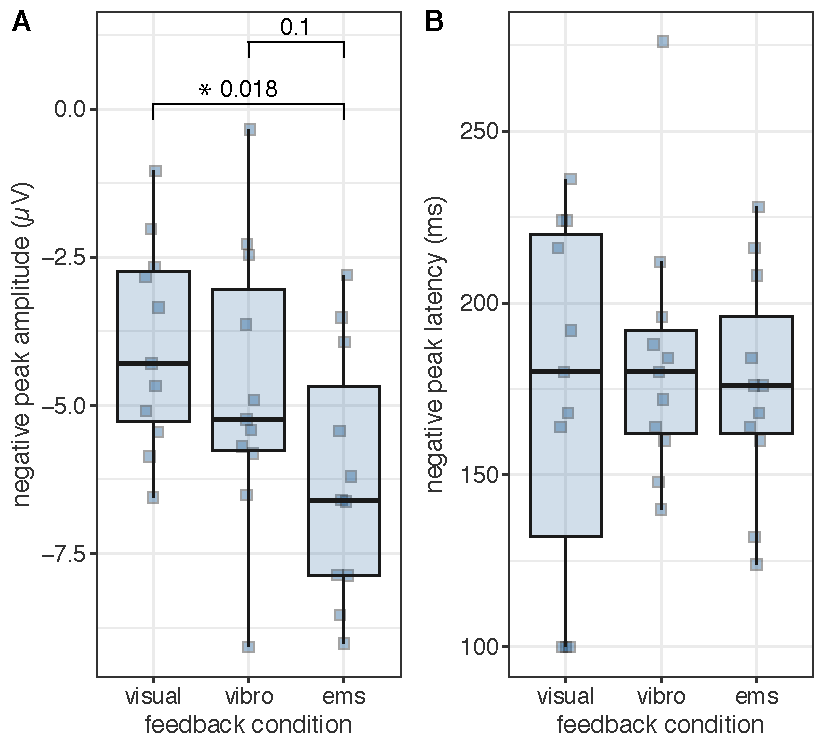
\includegraphics[width=\linewidth]{images/amplitude_and_latency.pdf}
\vspace{-10pt}
\caption{Negative peak amplitudes (in $\mu V$) and latencies (in ms) 100 to 300ms post object selection event in difference ERPs, see figure \ref{erp_diff}. Dots represent individual participants. Uncorrected p-values of pairwise comparisons were computed with non-parametric rank-sum tests.}
\label{erp_diff_stats}
\end{figure}

%In general, we considered significant results with $\alpha \leq 0.05$.





%\todo[inline]{THIS IS THE MAIN PART OF THE PAPER, let's spend our energy here.}

%\subsection{Reaction time results}
%\todo[]{same here, do not explain methods again in the results section. Also do let's not explain ERP and reaction time in the same section.}
%To further investigate changes in the accuracy of sensory-motor processing, here were interest in whether perception influences the accuracy of appropriate motor action behavior. We hypothesized participants to react quicker to haptic VR stimulation. We observed an expected increase in reaction time from the normal to the mismatch trials in all three conditions (on average $170ms$). Across the mismatch trials, reaction times when experiencing electrical muscle stimulation was lower ($mean = 220ms, sd = 100ms$) than for the vibration stimulation ($mean = 240 ms, sd = 70ms$) as well as the visual only condition ($mean = 260, sd = 60ms$). Furthermore, the reaction time correlated with the PEN amplitude ($/rho = .34, p = 0.06$) across haptic stimulation conditions providing first evidence for active sensory-motor processing.
%\begin{figure}[h!]
%\includegraphics[width=\linewidth]{images/paired_obs_erp_rt_line_FCz.pdf}
%\vspace{-10pt}
%\caption{}
%\label{task_flow}
%\end{figure}

\subsection{Questionnaire and users' comments}
%\missing{Sezen can you add the exit interview stuff here?}

First, as expected, we observed no significant differences in the level of immersion between conditions for any of the four IPQ questions we asked; this is likely caused by the experiment design, which contains randomly presented unrealistic trials that score very low on immersion.

Second, in the exit interviews, 8 participants voiced (that) they prefer the comfort and experience of the Vibro condition. Two participants preferred the EMS condition, stating it was ``more engaging''. One last participant stated that the visual condition was the most realistic condition but added ``it felt easier to perform the task in the EMS condition'' (likely due to the extra force feedback that informs of collision). 

%\begin{figure}[h!]
%\includegraphics[width=\linewidth]{images/ipq_rt.pdf}
%\vspace{-10pt}
%\caption{Level of immersion (IPQ) scores and time elapsed until movement stop of the hand after an object was selected (reaction time).}
%\label{task_flow}
%\end{figure}

%Correlation IPQ (G1 or mean of all scores) is not significant ($r = -0.08$ for the mean of all 4 items and $r = 0.09$ for the G1 item only)
%\begin{figure}[h!]
%\includegraphics[width=\linewidth]{images/paired_obs_ipq_erp_FCz.pdf}
%\vspace{-10pt}
%\caption{Level of immersion (IPQ) scores and time elapsed until movement stop of the hand after an object was selected (reaction time).}
%\label{task_flow}
%\end{figure}
\section{Contribution, Benefits \& Limitations}

With this study, we contributed a new approach to automatically detect conflicts in visuo-haptic sensory integration based on analyzing event-related brain potentials. We demonstrated in eleven participants using EEG recordings that our method is able to correctly detect prematurely given visuo-haptic feedback (combinations of visual, vibration and EMS). In the future, this approach might thus be used in combination with questionnaires such as IPQ or as an alternative measure that does not require interrupting the user.

We argue in favor of the scalability of our findings to complex environments: Successfully performing intended motor actions is the most fundamental way we interact with our environment. The ERP negativity paradigm relies on the fact that during well-known tasks (e.g. motor tasks) prediction errors elicit negative signals when the environment has a useful level of predictability. In fact, ERPs have been shown to model prediction mismatches in fairly complex setups such as: robotic arm control, driving, and gaming ~\cite{Salazar-Gomez2017,Chavarriaga2015,B.2018}. Furthermore, current trends in neuroadaptive technologies emphasize the scalability of these signals beyond simple tasks~\cite{zander_neuroadaptive_2016}. These findings suggest that this effect will be consistent in other, more complex, VR tasks that also require motor commands such as touching objects.

\subsection{Implications for the future of VR Research}

We believe that this is a first step towards a potential metric for visuo-haptic immersion based on detecting visuo-haptic mismatches. If follow up studies replicate the reported patterns of ERP modulation based on sensory mismatch, VR research will benefit four-fold: (1) evaluating haptic immersion via ERPs does not require interrupting the user's immersive experience to ask questions. (2) The latter will further enable to conduct background evaluations of the user's sense of haptic immersion, enabling new paradigms for user studies in VR (using implicit measures). (3) ERPs are not subject to the same degree of introspection as the standard presence questionnaires. (4) This technique can be used as the building-block for VR applications that want to automatically adjust to the user's perception of conflicts, e.g., using our approach, an application could automatically adjust collision detection volumes based on the user's ERPs. 

%, (3) as companies start to offer VR headsets with embedded EEG-devices (such as LooxidVR), we believe this metric can be used to assess the level of immersion of a user in realtime, so that the VR application can adjust the haptic feedback automatically to best serve the user, without needing to stop and ask "calibration questions". 

\subsection{Limitations}
As with any system based on EEG, our approach has its inherent shortcomings: (1) ERP data is typically not taken per-trial but averaged over many trials and thus require high number of trial repetitions. In addition, (2) high-resolution EEG is still cumbersome to apply and requires time and expertise. However, researchers are working towards single-trial ERP analysis approaches ~\cite{blankertz_single-trial_2011}, and we do believe that new EEG systems will be directly embedded in future VR headsets allowing easy setup and recording of electrophysiological signals~\footnote{\label{VREEG}\url{http://looxidlabs.com/product/}, last accessed on 18/09/2018.} with new comfortable electrode types~\cite{nikulin_miniaturized_2010}, including dry electrodes~\cite{zander_evaluation_2017}. These EEG limitations put a cap on using our approach for quickly iterating on the design of a haptic VR scene. However, when designers want to develop and validate haptic immersion in VR scenarios without interrupting the user, our approach could, in the future offer, a potential replacement for questionnaires.
\section{Conclusions}

In this paper, we propose a technique that allows us to detect haptic conflicts in VR, which is based on event-related brain potentials obtained using EEG during interaction with virtual objects. We found out in our user study that the early negativity component of the ERP (the prediction error) is more pronounced during situations with haptic conflicts, such as: inadequate or delayed haptic feedback, poorly configured collision detection, etc. This result suggests we can successfully detect haptic conflicts using our proposed technique. In fact, we found out that, when the number of mismatched feedback channels increases, the prediction error increases.

Thus, we believe this is a first step to establish the potential of ERPs as an indicator for visuo-haptic mismatches in VR. We discussed the impact of our findings for VR research and lay out two potential avenues to this future metric: a complement to the traditional presence questionnaires or an alternative metric that does not require interrupting the user.

As for future work, we plan two courses of action, a technical and an experimental angle. First, we plan to explore a real-time implementation of our analysis scripts, which would enable real-time adaptation of the haptic devices based on the user's ERPs (e.g., inspired by recent work in EEG-based adaptive VR~\cite{zander_evaluation_2017}); to achieve this we will explore implementing our scripts into a real-time EEG-based cloud service, such as intheon\footnote{\url{https://intheon.io}, last accessed 17/09/2018}. Secondly, while we believe our work is a first step, more research is required to solidify ERPs as a metric for haptic immersion; for instance, one needs to explore how sensitive the prediction error is to different sensory channels beyond vibration and EMS. 

Lastly, our work might fuel a new investigation into the uncanny valley of haptics~\cite{Berger2018}. Specifically, one might investigate at what perceptual threshold does haptic feedback negatively impact the accuracy of user's predictions of a virtual environment? 

\begin{acks}
We kindly thank our colleague Jas Brooks at the University of Chicago for helping us proofread this work.
\end{acks}


\bibliographystyle{ACM-Reference-Format}
\bibliography{bibliography}

%\newpage
%\todototoc
%\listoftodos

\end{document}
